\documentclass[a4paper, 12pt, oneside]{report}
% ─── Шрифты и язык ────────────────────────────────────────────
\usepackage{fontspec}
\usepackage[main=russian, english]{babel}
\setmainfont{Times New Roman}

% ─── Кегль основного текста: 13пт (ГОСТ 7.32-2017 допускает 12--14) ──
\renewcommand{\normalsize}{\fontsize{13}{15.6}\selectfont}
\normalsize

% ─── Поля страницы (ГОСТ 7.32-2017) ──────────────────────────
\usepackage{geometry}
\geometry{
  a4paper,
  left   = 30mm,
  right  = 15mm,
  top    = 20mm,
  bottom = 20mm
}

% ─── Межстрочный интервал и отступ ───────────────────────────
\usepackage{setspace}
\onehalfspacing
\usepackage{indentfirst}
\setlength{\parindent}{1.25cm}

% ─── Математика ───────────────────────────────────────────────
\usepackage{amsmath, amssymb}

% ─── Графика ─────────────────────────────────────────────────
\usepackage{graphicx}
\graphicspath{{../sch/}{../../py/figures/}}
\usepackage{float}

% ─── Таблицы ─────────────────────────────────────────────────
\usepackage{booktabs}
\usepackage{array}

% ─── Ссылки ──────────────────────────────────────────────────
\usepackage[hidelinks]{hyperref}
\usepackage{url}

% ─── Подписи к рисункам и таблицам (ГОСТ) ────────────────────
\usepackage{caption}
\DeclareCaptionLabelSeparator{emdash}{~---~}
\captionsetup[figure]{
  name      = Рисунок,
  labelsep  = emdash,
  justification = centering,
  position  = below,
  font      = normalsize
}
\captionsetup[table]{
  name      = Таблица,
  labelsep  = emdash,
  justification = raggedright,
  singlelinecheck = false,
  position  = top,
  font      = normalsize
}

% ─── Сквозная нумерация рисунков и таблиц ────────────────────
\usepackage{chngcntr}
\counterwithout{figure}{chapter}
\counterwithout{table}{chapter}

% ─── Заголовки разделов (ГОСТ) ───────────────────────────────
\usepackage{titlesec}

\titleformat{\chapter}[block]
  {\centering\normalfont\fontsize{14}{16.8}\selectfont\bfseries}
  {\thechapter.}{0.5em}{}
\titlespacing*{\chapter}{0pt}{0pt}{14pt}

\titleformat{\section}[block]
  {\normalfont\fontsize{14}{16.8}\selectfont\bfseries}
  {\thesection.}{0.5em}{}
\titlespacing*{\section}{0pt}{14pt}{6pt}

\titleformat{\subsection}[block]
  {\normalfont\fontsize{13}{15.6}\selectfont\bfseries}
  {\thesubsection.}{0.5em}{}
\titlespacing*{\subsection}{0pt}{12pt}{4pt}

% ─── Колонтитулы и нумерация страниц ─────────────────────────
\usepackage{fancyhdr}
\pagestyle{fancy}
\fancyhf{}
\fancyfoot[C]{\thepage}
\renewcommand{\headrulewidth}{0pt}
\renewcommand{\footrulewidth}{0pt}
\fancypagestyle{plain}{%
  \fancyhf{}%
  \fancyfoot[C]{\thepage}%
  \renewcommand{\headrulewidth}{0pt}%
}

% ─── Оглавление ───────────────────────────────────────────────
\usepackage{tocloft}
\renewcommand{\cfttoctitlefont}{\hfill\normalfont\fontsize{14}{16.8}\bfseries}
\renewcommand{\cftaftertoctitle}{\hfill}
\setlength{\cftbeforechapskip}{4pt}
\setlength{\cftbeforesecskip}{0pt}

% ─── Нумерация формул по главам ───────────────────────────────
\numberwithin{equation}{chapter}

% ─── Списки ───────────────────────────────────────────────────
\usepackage{enumitem}
\setlist{itemsep=2pt, topsep=4pt}
\setlist[enumerate]{label=\arabic*), leftmargin=\parindent}
\setlist[itemize]{leftmargin=\parindent}

% ─── Библиография ─────────────────────────────────────────────
\renewcommand{\bibname}{Список использованных источников}
\makeatletter
\renewcommand\@biblabel[1]{#1.}   % [1] → 1.
\makeatother

% ─── TikZ (для схемы маршрута) ────────────────────────────────
\usepackage{tikz}
\usetikzlibrary{positioning, arrows.meta}


\begin{document}

%% ============================================================
%%  ТИТУЛЬНЫЙ ЛИСТ
%% ============================================================
\begin{titlepage}
  \thispagestyle{empty}
  \begin{center}
    {\small
    Министерство науки и высшего образования Российской Федерации\\[2pt]
    Федеральное государственное автономное образовательное учреждение\\
    высшего образования\\[4pt]
    \textbf{«Московский физико-технический институт\\
    (национальный исследовательский университет)»}\\[6pt]
    Физтех-школа радиотехники и компьютерных технологий\\[2pt]
    Кафедра мультимедийных технологий и телекоммуникаций
    }
  \end{center}

  \vspace{1.8cm}

  \begin{center}
    \textbf{ВЫПУСКНАЯ КВАЛИФИКАЦИОННАЯ РАБОТА}\\[4pt]
    \textit{(бакалаврская работа)}\\[12pt]
    по направлению подготовки «Прикладная математика и физика»\\[10pt]
    на тему:\\[8pt]
    {\large\textbf{«Снижение энергопотребления умножителя Бута\\
    в адаптивном цифровом фильтре\\
    за счёт методов перекодировки»}}
  \end{center}

  \vfill

  \begin{flushright}
    \begin{tabular}{ll}
      Студент группы Б01-205:    & Сажнев М.\,Е.\\[8pt]
      Научный руководитель:       & Соловьев Д.\,М.\\
    \end{tabular}
  \end{flushright}

  \vspace{2cm}

  \begin{center}
    Долгопрудный, 2026
  \end{center}
\end{titlepage}

%% ============================================================
%%  АННОТАЦИЯ
%% ============================================================
\chapter*{Аннотация}
\addcontentsline{toc}{chapter}{Аннотация}

Работа посвящена снижению энергопотребления умножителя Бута radix-4 в
адаптивных цифровых фильтрах за счёт вынесенного перекодировщика,
дополненного методом перекодировки для увеличения числа нулевых частичных 
произведений.
Предложена архитектура, в которой блок кодировки Бута и перекодировщик
выносятся за пределы умножителя и выполняются однократно при обновлении
коэффициента фильтра. Архитектура реализована на языке Verilog и
верифицирована функционально. Площадь умножителя практически не
изменилась ($\Delta < 0{,}3\%$). Потребляемая мощность в реалистичном
сценарии снижена на $2{,}9\%$ при отношении сигнал/шум $52\,\text{дБ}$ и
нулевом систематическом смещении~--- что соответствует требованиям
большинства задач цифровой обработки сигналов. Маршрут измерений
построен целиком на открытых инструментах: Yosys, Icarus~Verilog,
OpenSTA, библиотека NanGate45 (45~нм).

\vspace{0.5em}
\textit{Ключевые слова:} умножитель Бута, приближённые вычисления,
перекодировка, адаптивные FIR-фильтры, энергопотребление.

%% ============================================================
%%  СОДЕРЖАНИЕ
%% ============================================================
\tableofcontents

%% ============================================================
%%  ОБОЗНАЧЕНИЯ И СОКРАЩЕНИЯ
%% ============================================================
\chapter*{Обозначения и сокращения}
\addcontentsline{toc}{chapter}{Обозначения и сокращения}

\begin{tabular}{@{}ll}
  ЦОС     & цифровая обработка сигналов \\
  FIR     & \textit{finite impulse response} --- фильтр с конечной импульсной характеристикой \\
  LMS     & \textit{least mean squares} --- алгоритм наименьших средних квадратов \\
  RTL     & \textit{register transfer level} --- уровень регистровых передач \\
  VCD     & \textit{value change dump} --- формат записи активности сигналов \\
  NMED    & \textit{normalized mean error distance} --- нормированное среднее расстояние ошибки \\
  MRED    & \textit{mean relative error distance} --- среднее относительное расстояние ошибки \\
  SNR     & \textit{signal-to-noise ratio} --- отношение сигнал/шум \\
  ED      & \textit{error distance} --- расстояние ошибки \\
  ER      & \textit{exact recoding} --- точная перекодировка \\
  AR      & \textit{approximate recoding} --- приближённая перекодировка \\
  PP      & \textit{partial product} --- частичное произведение \\
\end{tabular}

%% ============================================================
%%  ВВЕДЕНИЕ
%% ============================================================
\chapter*{Введение}
\addcontentsline{toc}{chapter}{Введение}

Умножители занимают центральное место в задачах цифровой обработки
сигналов (ЦОС): фильтрации, преобразования Фурье, адаптивных систем
управления и нейросетевого инференса. В современных цифровых схемах
умножитель является одним из наиболее затратных блоков как по занимаемой
площади кристалла, так и по потребляемой мощности. Это особенно
критично в приложениях реального времени, таких как адаптивные
FIR-фильтры: в $N$-тапном фильтре умножение выполняется на каждом тапе
при каждом входном отсчёте, и умножитель доминирует в
энергобюджете системы.

Обоснование применимости приближённых вычислений в ЦОС опирается в
первую очередь на
принципиальное ограничение точности самих входных сигналов. В типичных
приложениях~--- обработке речи, звука и радиолокационных
сигналов~--- входной сигнал неизбежно содержит шум. Типичное отношение
сигнал/шум (SNR) составляет 30--60~дБ. Это означает, что биты
арифметического результата, соответствующие погрешности ниже уровня
шума сигнала, не несут практически значимой информации: стандартная
16-битная точность (${\approx}96\,\text{дБ}$) существенно избыточна.
Данное обстоятельство открывает путь к \textit{приближённым
вычислениям}: сознательному допущению малых арифметических погрешностей
ради снижения сложности и энергопотребления.

Базовым методом оптимизации умножителей служит алгоритм
Бута~radix-4~\cite{booth1951}: он вдвое сокращает число частичных
произведений по сравнению с прямым двоичным умножением. Zhu~и~соавт.~\cite{zhu2025} предложили метод, дополнительно
увеличивающий долю \textit{нулевых} частичных произведений за счёт
перекодировки соседних кодов Бута. Нулевые строки в
матрице частичных произведений, полученные в результате перекодировки
коэффициентов Бута приводят к меньшему числу переключений в модуле 
финального сложения, что напрямую снижает динамическую мощность.

Тем не менее прямое применение этого метода в адаптивном FIR-фильтре
сопряжено с рядом архитектурных препятствий, подробно рассмотренных в
настоящей работе. Предлагаемое решение обходит эти препятствия путём
выноса блока перекодировки за пределы умножителя с амортизацией его
стоимости по числу умножителей в одном фильтре.

\textbf{Цель работы}~--- снизить энергопотребление умножителя Бута в
адаптивном цифровом фильтре, применив методы перекодировки с
добавлением нулевых кодов.

\textbf{Задачи:}
\begin{enumerate}
  \item Адаптировать алгоритм перекодировки~\cite{zhu2025}
        к параллельной архитектуре умножителя.
  \item Предложить архитектурное решение, реализующее преимущества
        перекодировки в сценарии адаптивного фильтра.
  \item Реализовать предложенную архитектуру на языке описания
        аппаратуры Verilog.
  \item Построить методику измерения площади и мощности на
        общедоступных инструментах (45~нм).
  \item Оценить точность приближённых режимов по метрикам NMED, MRED,
        SNR на статистике $10^6$~пар.
\end{enumerate}

%% ============================================================
%%  ГЛАВА 1
%% ============================================================
\chapter{Предметная область}

\section{Умножитель Бута radix-4}

Алгоритм Бута radix-4~\cite{booth1951} основан на разбиении
$n$-битного множителя~$A$ (в дополнительном коде) на перекрывающиеся
группы по 3~бита с шагом~2:
\[
  \bigl(a_{2i+1},\; a_{2i},\; a_{2i-1}\bigr),
  \qquad i = 0, 1, \ldots, n/2 - 1, \quad a_{-1} \triangleq 0.
\]
Каждая тройка кодируется одним значением из набора
$M_i \in \{-2, -1, 0, +1, +2\}$ и представляется тремя управляющими
значениями:
\begin{itemize}
  \item \texttt{neg}~--- знак ($M_i < 0$);
  \item \texttt{one}~--- $|M_i| = 1$;
  \item \texttt{two}~--- $|M_i| = 2$.
\end{itemize}
Итого получается $n/2$~кодов Бута~--- вдвое меньше частичных
произведений (PP), чем при прямом умножении. Каждый код порождает
одну строку в матрице PP:
\[
  P_i = M_i \cdot B \cdot 2^{2i},
\]
где $B$~--- второй операнд, а множитель $2^{2i}$ отражает вес
$i$-й группы: поскольку группы сформированы с шагом~2, каждый
следующий код Бута соответствует сдвигу множителя на~2~разряда
влево, то есть умножению на~$4^i = 2^{2i}$. Итоговое произведение
получается суммой $\sum_i P_i$ в дереве Уоллеса или Дадды.

Нулевой код Бута ($M_i = 0$) даёт строку $P_i \equiv 0$: она не
вносит вклада в сумму и не создаёт переключений сигналов в
суммирующем дереве. Именно эта особенность является основой метода
перекодировки, рассматриваемого в главе~2.

В данной работе рассматривается 16-битный умножитель в дополнительном
коде, дающий $n/2 = 8$~кодов Бута и 32-битный результат. Схема
умножителя представлена на рисунке~\ref{fig:booth_mult}.

\begin{figure}[H]
  \centering
  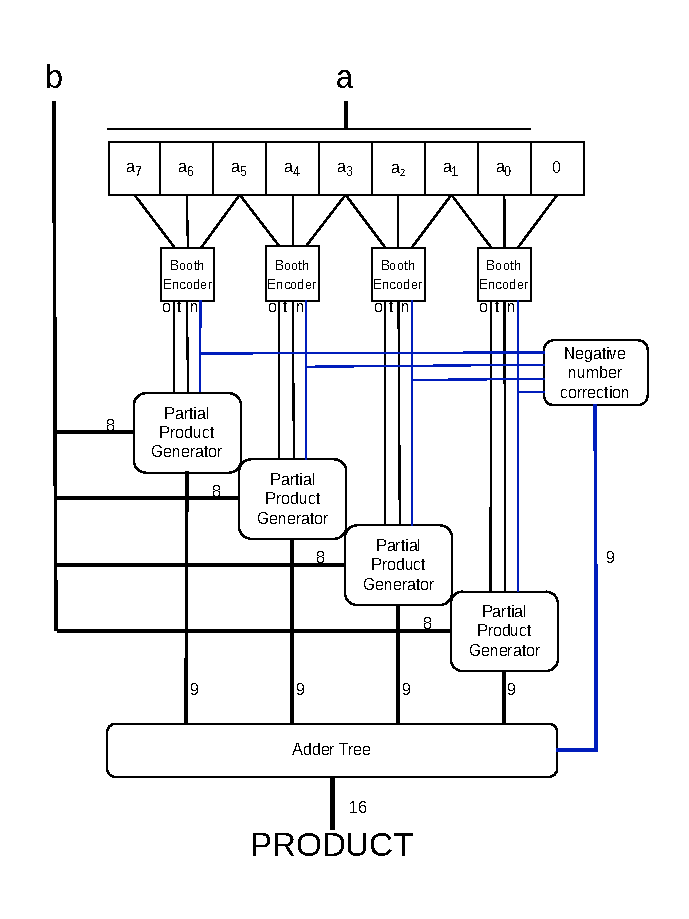
\includegraphics[width=0.55\textwidth]{booth_mult.pdf}
  \caption{Схема умножителя Бута radix-4. Пример для восьмибитных чисел.}
  \label{fig:booth_mult}
\end{figure}

\section{Адаптивный FIR-фильтр}

$N$-тапный адаптивный FIR-фильтр вычисляет выходной сигнал по формуле:
\begin{equation}
  y[n] = \sum_{k=0}^{N-1} w_k[n] \cdot x[n-k],
  \label{eq:fir}
\end{equation}
где $x[n]$~--- входной отсчёт, а $w_k[n]$~--- коэффициенты фильтра,
обновляемые адаптивным алгоритмом (например, LMS)~\cite{haykin2013}.

Ключевая особенность структуры~(\ref{eq:fir})~--- \textit{асимметрия
темпов обновления} двух операндов каждого умножителя:
\begin{itemize}
  \item входной отсчёт $x[n]$ меняется \textbf{каждый такт};
  \item коэффициент $w_k[n]$ обновляется \textbf{редко}~--- раз в
        $10$--$10^3$~тактов, в зависимости от скорости сходимости
        алгоритма. Данная асимметрия является ключевым ресурсом 
        для предлагаемой архитектурной оптимизации.
\end{itemize}


\section{Приближённые вычисления в задачах ЦОС}

Обоснование применимости приближённых вычислений в ЦОС опирается на
следующее наблюдение: \textit{точность, необходимая для вычислений, не
должна превышать точность исходных данных}. Сигналы в прикладных
системах изначально зашумлены, например это может это может быть шум квантования
записывающего устройства, если речь идет про звук, или шум, добавляющийся при 
прохождении сигнала через канал связи. Типичный диапазон SNR входного сигнала:

\begin{itemize}
  \item телефонная речь: 30--40~дБ;
  \item аудио высокого качества: 50--70~дБ;
  \item радиолокационный сигнал: 10--40~дБ.
\end{itemize}

Стандартное 16-битное арифметическое умножение обеспечивает точность
около 96~дБ~--- существенно выше уровня шума в перечисленных
приложениях. Иными словами, младшие биты результата умножения несут
информацию о сигнале с точностью, которая уже скрыта за уровнем
шума: отличить «правильный» результат от «приближённого» на фоне
этого шума невозможно. Таким образом, смысла в арифметической
точности выше уровня шума сигнала нет, и можно намеренно допустить
небольшую арифметическую погрешность, лишь бы она не превышала
этот уровень.

%% ============================================================
%%  ГЛАВА 2
%% ============================================================
\chapter{Метод перекодировки для создания нулевых частичных произведений}

\section{Алгоритм перекодировки}

Авторы~\cite{zhu2025} вводят вспомогательную переменную~$x$ и предлагают
заменить пару соседних кодов Бута $M_{2i+1}$, $M_{2i}$ парой
$K_{2i+1}$, $K_{2i}$ по формулам:
\begin{equation}
  K_{2i+1} = M_{2i+1} - x,
  \qquad
  K_{2i}   = M_{2i} + 4\,x.
  \label{eq:recoding}
\end{equation}
Данное преобразование сохраняет суммарный вклад пары в произведение:
\[
  K_{2i+1}\cdot 4^{2i+1} + K_{2i}\cdot 4^{2i}
  = (M_{2i+1} - x)\cdot 4^{2i+1} + (M_{2i} + 4x)\cdot 4^{2i}
  = M_{2i+1}\cdot 4^{2i+1} + M_{2i}\cdot 4^{2i},
\]
поскольку $4\cdot 4^{2i} = 4^{2i+1}$.
Полагая $x = M_{2i+1}$, получаем $K_{2i+1} = 0$~---
код первой пары обнуляется, а второй принимает значение
$K_{2i} = M_{2i} + 4\,M_{2i+1}$.

\begin{figure}[H]
  \centering
  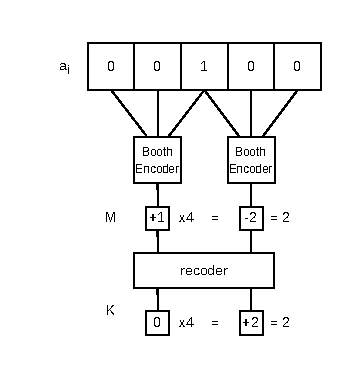
\includegraphics[width=0.48\textwidth]{recoding.pdf}
  \caption{Пример точной перекодировки (ER): $M_{2i+1}=+1$, $M_{2i}=-2$
           переходят в $K_{2i+1}=0$, $K_{2i}=+2$}
  \label{fig:recoding}
\end{figure}

Перекодировка срабатывает, если пятибитный паттерн
$a_{2i+3}\,a_{2i+2}\,a_{2i+1}\,a_{2i}\,a_{2i-1}$ принадлежит
одному из наборов, приведённых в таблице~\ref{tab:patterns}.

\begin{table}[H]
  \caption{Паттерны перекодировки: значения кодов Бута до и после
           преобразования}
  \label{tab:patterns}
  \centering
  \renewcommand{\arraystretch}{1.3}
  \begin{tabular}{clrrrrc}
    \toprule
    Режим & Паттерн & $M_{2i+1}$ & $M_{2i}$ & $K_{2i+1}$ & $K_{2i}$
          & $\mathrm{ED}$ \\
    \midrule
    ER & \texttt{00100} & $+1$ & $-2$ & $0$ & $+2$   & $0$  \\
    ER & \texttt{11011} & $-1$ & $+2$ & $0$ & $-2$   & $0$  \\
    AR & \texttt{00101}, \texttt{00110} & $+1$ & $-1$ & $0$ & $+2^*$ & $+1$ \\
    AR & \texttt{11001}, \texttt{11010} & $-1$ & $+1$ & $0$ & $-2^*$ & $-1$ \\
    \bottomrule
  \end{tabular}
  \\[4pt]
  \raggedright\small
  ${}^*$Точное значение $K_{2i} = \pm3$ выходит за диапазон кодов Бута
  и округляется до $\pm2$; разность~1 составляет погрешность~$\mathrm{ED}$.
\end{table}

В точном режиме (ER) перекодировка обнуляет~$K_{2i+1}$ без ошибки.
В приближённом режиме (AR) к этому добавляются ещё 4~паттерна~---
погрешность составляет~$\mathrm{ED} = \pm 1$ на одно частичное
произведение.

\section{Реализованные режимы перекодировки}

Во всех пяти режимах распознаётся один и тот же набор из шести паттернов:
два точных (ER: \texttt{00100}, \texttt{11011}) и четыре приближённых
(AR: \texttt{00101}, \texttt{00110}, \texttt{11001}, \texttt{11010}).
Различие между режимами состоит в том, в каких позициях коэффициента
разрешено применять AR.

При 16-битном коэффициенте алгоритм Бута radix-4 образует 8~пар с
индексами $i = 0$ (наименее значимая) до $i = 7$ (наиболее значимая).
Ошибка приближённого перекодирования на паре~$i$ добавляет погрешность
$\pm B\cdot 4^i$ к итоговому произведению: чем старше пара, тем
крупнее последствия ошибки. Точная перекодировка~(ER) разрешена в любой
паре во всех режимах. Приближённая~(AR) ограничивается только несколькими
\textit{младшими} парами, которых становится больше с ростом номера режима:

\begin{itemize}
  \item \textbf{\texttt{exact}}~--- AR не применяется ни в одной паре;
        результат математически точен.
  \item \textbf{\texttt{approx\_1}}~--- AR разрешена в парах $i < 2$
        (2~младшие пары, биты коэффициента $a_3$--$a_0$).
  \item \textbf{\texttt{approx\_2}}~--- AR разрешена в парах $i < 4$
        (4~младшие пары, биты $a_7$--$a_0$).
  \item \textbf{\texttt{approx\_3}}~--- AR разрешена в парах $i < 6$
        (6~младших пар, биты $a_{11}$--$a_0$).
  \item \textbf{\texttt{approx\_4}}~--- AR разрешена во всех 8~парах.
\end{itemize}

На каждое отдельное срабатывание AR погрешность составляет $\mathrm{ED} = \pm 1$
относительно данной пары. Однако суммарная погрешность произведения растёт
с номером режима: более высокие режимы допускают ошибки в старших парах,
вес которых $4^i$ существенно больше.

Важное конструктивное свойство: паттерны \texttt{00101/00110} дают
$\mathrm{ED} = +1$, а \texttt{11001/11010}~--- $\mathrm{ED} = -1$. Эти
паттерны противоположны, и при случайных данных встречаются примерно
одинаково часто. Поэтому систематическое смещение результата близко к
нулю, и погрешность не накапливается при длительной работе.

\section{Статистический анализ доли нулевых строк}

Эффективность метода зависит от того, как часто паттерны
перекодировки встречаются в реальных данных. На рисунке~\ref{fig:patterns}
показана средняя доля нулевых строк матрицы PP для каждого режима,
оценённая на выборке из $10^6$~пар с равномерным и гауссовым
распределениями входных данных.

\begin{figure}[H]
  \centering
  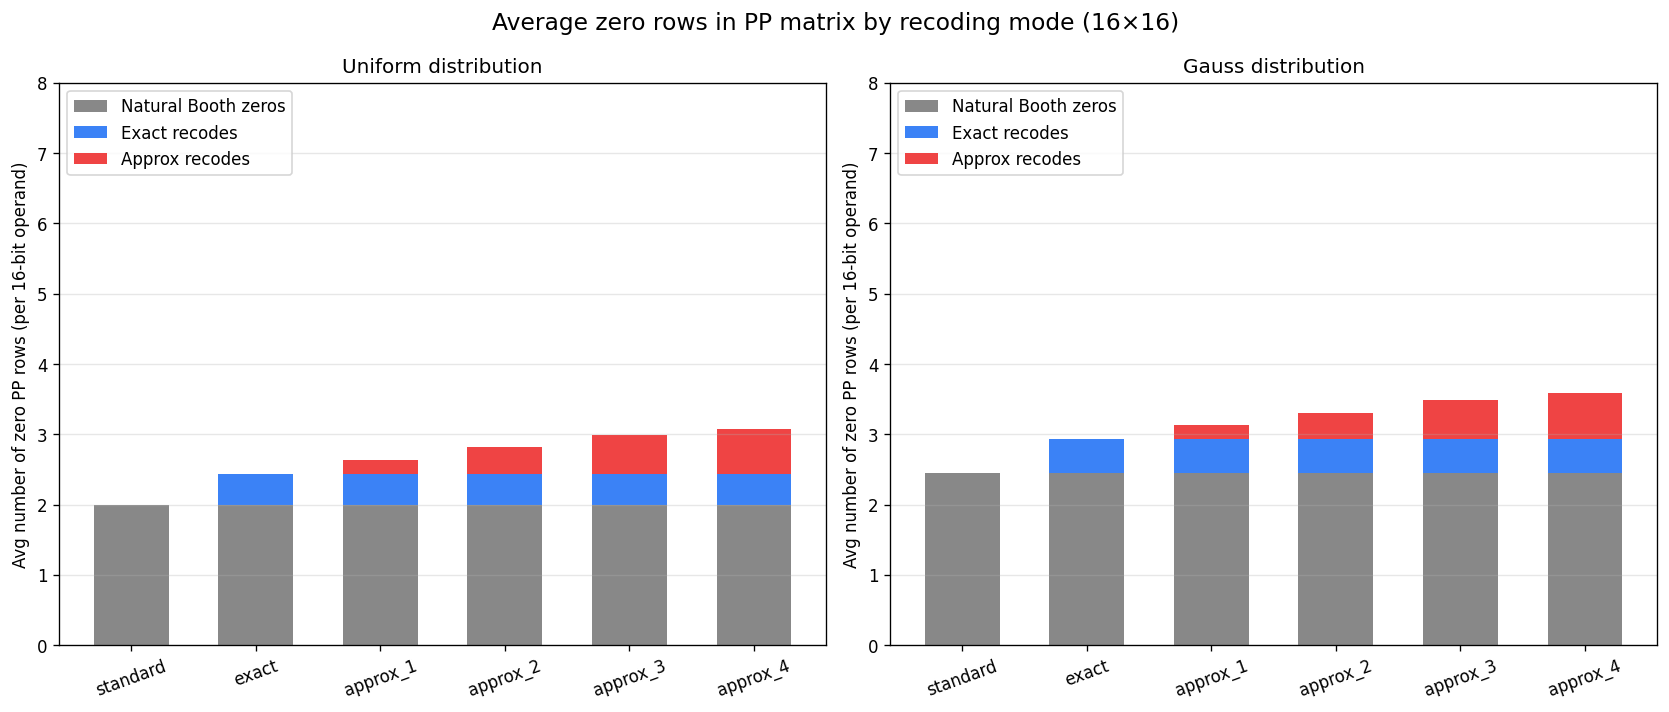
\includegraphics[width=0.9\textwidth]{patterns_zero_rows_by_mode.png}
  \caption{Средняя доля нулевых строк матрицы частичных произведений
           по режимам перекодировки}
  \label{fig:patterns}
\end{figure}

Доля нулевых строк монотонно возрастает с уровнем приближения. Для
режима \texttt{approx\_2} она существенно выше, чем для \texttt{exact},
что и обеспечивает дополнительную экономию мощности при умеренной погрешности.

%% ============================================================
%%  ГЛАВА 3
%% ============================================================
\chapter{Архитектура с вынесенным перекодировщиком}

\section{Проблемы прямого применения метода}

Метод~\cite{zhu2025} был разработан для \textit{последовательного}
умножителя: на каждом такте вычисляется одно частичное произведение и
прибавляется к общей сумме, если коэффициент Бута оказывается нулевым,
то сложение пропускается. Это позволяет экономить тактовые циклы за
счёт переменного числа шагов.

Такой подход неприменим в потоковом FIR-фильтре. Каждый умножитель в
фильтре обязан выдавать результат \textit{каждый такт}: переменная
задержка потребовала бы межумножительного контроллера готовности,
накладные расходы которого перекрыли бы весь выигрыш. Кроме того,
потоковые задачи ЦОС требуют фиксированной пропускной способности,
несовместимой с последовательной архитектурой.

Схема конфликта показана на рисунке~\ref{fig:problem}: умножители 
завершают работу за разное число тактов, из-за чего происходит
рассинхронизация.

\begin{figure}[H]
  \centering
  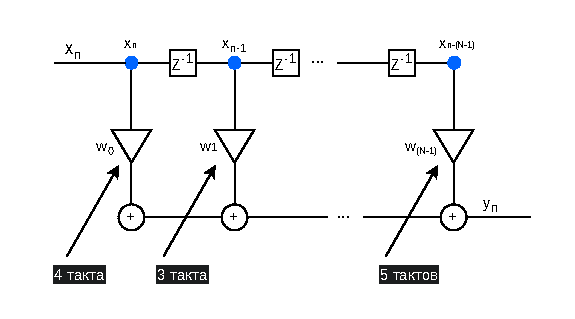
\includegraphics[width=0.68\textwidth]{problem.pdf}
  \caption{Проблема последовательного умножителя в конвейере
           FIR-фильтра}
  \label{fig:problem}
\end{figure}

Таким образом, метод необходимо адаптировать к параллельному умножителю
с фиксированной однотактной задержкой.

\section{Проблема размещения перекодировщика внутри умножителя}

Очевидным первым шагом кажется размещение перекодировщика~(\ref{eq:recoding})
перед блоком генерации частичных произведений внутри параллельного
умножителя. Однако это наталкивается на принципиальное ограничение:
алгоритм перекодировки обрабатывает пары кодов Бута
\textit{последовательно}, справа налево.

Причина~--- перекрывание пятибитных паттернов (рисунок~\ref{fig:sequential}):
каждый коэффициент участвует в перекодировании дважды, поэтому перекодировка
новой пары невозможна, пока не будет произведена перекодировка предыдущей.


\begin{figure}[H]
  \centering
  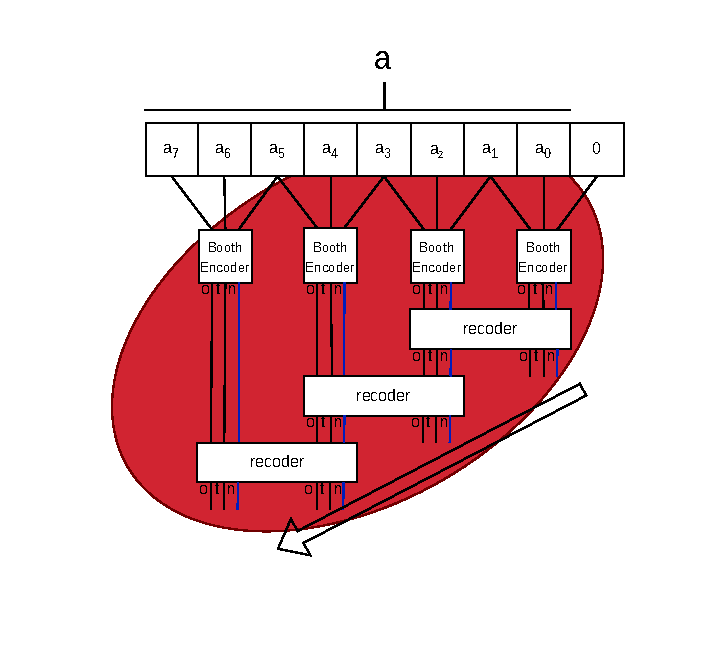
\includegraphics[width=0.68\textwidth]{sequential.pdf}
  \caption{Последовательная зависимость между парами в алгоритме
           перекодировки. Пример для 8-битного числа.}
  \label{fig:sequential}
\end{figure}

Возможен вариант, когда рассматриваются только непересекающиеся пары. Но 
в таком случае число попыток для перекодировки снижается примерно вдвое.

Кроме того, перекодировщик~--- это дополнительная комбинационная
логика, которая сама потребляет динамическую мощность при каждом
умножении. В $N$-тапном фильтре с $N$~умножителями перекодировщик
размножился бы в $N$~экземпляров. Таким образом, простое добавление
перекодировщика внутрь параллельного умножителя увеличивает мощность,
а не снижает её.

\section{Предлагаемая архитектура}

Предлагаемое решение использует асимметрию скоростей обновления,
описанную в разделе~1.2. Коэффициент $w_k$ обновляется редко~---
следовательно, на скорость вычисления этого коэффициента не накладывается
жестких временных ограничений. В таком случае можно применять 
последовательный алгоритм перекодировки для всех пересекающихся пар.
Кроме того, один и тот же модуль можно использовать для вычисления 
коэффициентов сразу нескольких умножителей внутри одного фильтра. Таким 
образом стоимость вынесенного кодировщика будет разделена на число 
умножителей, для которых он производит вычисления. 

Архитектура строится на четырёх принципах:
\begin{enumerate}
  \item \textbf{Вынесение.} Блок кодировки Бута и перекодировщик
        выносятся за пределы умножителя в отдельный аппаратный модуль.
  \item \textbf{Однократное вычисление.} Перекодировка выполняется
        один раз при каждом обновлении коэффициента~--- без ограничений
        реального времени.
  \item \textbf{Хранение.} Результирующий 24-битный вектор
        $\{\texttt{two}[7:0],\; \texttt{one}[7:0],\; \texttt{neg}[7:0]\}$
        записывается в регистр умножителя вместо исходного
        16-битного коэффициента.
  \item \textbf{Единый RTL.} Сам умножитель одинаков для всех режимов
        точности; выбор режима определяется только содержимым 
        перекодированных коэффициентов, записанных в регистры.
\end{enumerate}

Сравнение базовой и предлагаемой схем умножителя приведено на
рисунке~\ref{fig:extrec}.

\begin{figure}[H]
  \centering
  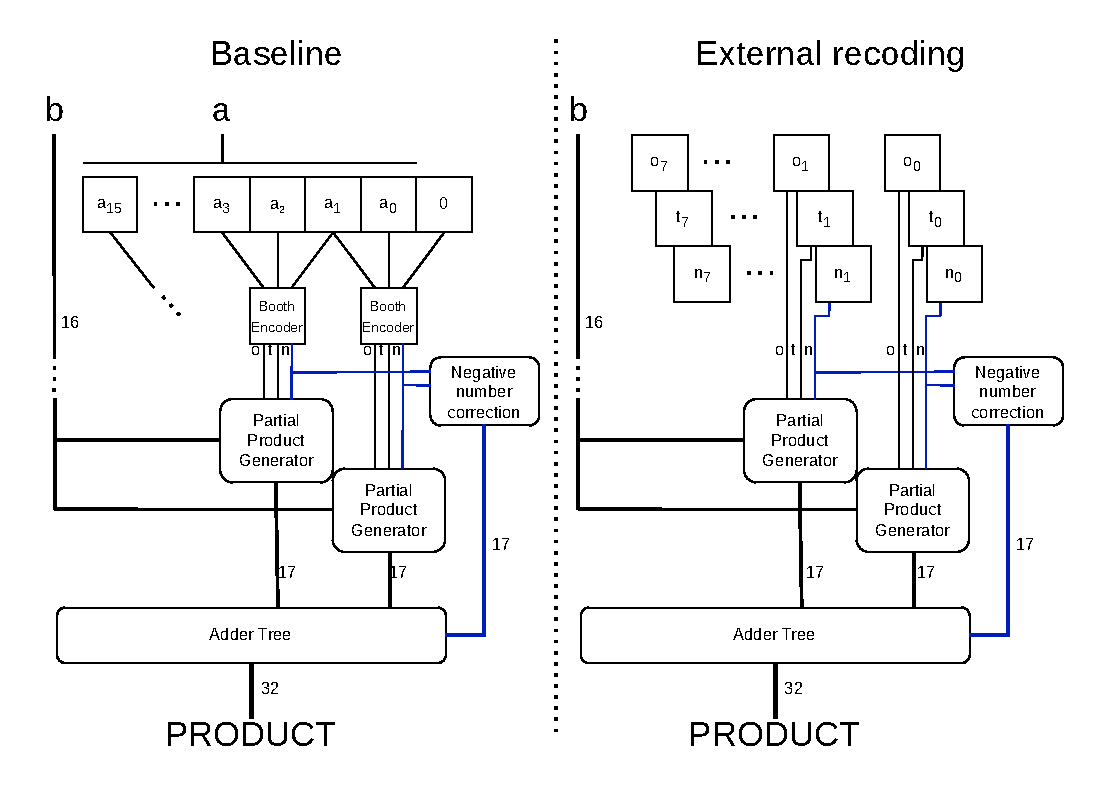
\includegraphics[width=\textwidth]{extrec.pdf}
  \caption{Базовая схема (слева): перекодировщик внутри умножителя.
           Предлагаемая схема (справа): перекодировщик вынесен наружу,
           умножитель принимает готовый вектор}
  \label{fig:extrec}
\end{figure}

%% ============================================================
%%  ГЛАВА 4
%% ============================================================
\chapter{Реализация и методика измерений}

\section{RTL-реализация}

Разработаны два RTL-модуля на языке Verilog:
\begin{itemize}
  \item \textbf{\texttt{mult\_booth}}~--- исходный умножитель:
        radix-4 Booth с перекодировщиком \textit{внутри}.
        Используется как базовый вариант для сравнения.
  \item \textbf{\texttt{mult\_booth\_extrec}}~--- предлагаемый
        умножитель: принимает готовый 24-битный вектор управляющих
        сигналов \{\texttt{two}, \texttt{one}, \texttt{neg}\}.
        Логики кодирования не содержит.
\end{itemize}

Оба модуля реализуют 16$\times$16-битное знаковое умножение
(дополнительный код), выдают 32-битный результат за один такт
и синтаксически идентичны в части итогового суммирующего дерева.

\section{Программный перекодировщик}

Перекодировщик реализован на языке Python. Алгоритм последовательно
обрабатывает все 7~пар пятибитных паттернов 16-битного множителя
и генерирует 24-битный управляющий вектор. Поддерживаются все пять
режимов: \texttt{exact} и \texttt{approx\_1}--\texttt{approx\_4}.

Результат записывается в регистр аппаратного умножителя через
интерфейс конфигурации. При необходимости аппаратной реализации
алгоритм может быть перенесён в RTL без изменений в самом умножителе.

\section{Маршрут синтеза и анализа мощности}

Маршрут целиком построен на открытых инструментах и общедоступной
библиотеке стандартных ячеек. Этапы показаны на
рисунке~\ref{fig:flow}.

\begin{enumerate}
  \item \textbf{Генерация стимулов.} Python-перекодировщик формирует
        файлы пар $(a,\,b)$ и соответствующих перекодированных
        векторов для заданного тестового сценария.
  \item \textbf{Синтез.} Yosys~--- открытый инструмент синтеза RTL~---
        транслирует Verilog-описание в gate-level нетлист,
        отображённый на стандартные ячейки библиотеки
        NanGate45~--- открытой академической библиотеки
        технологической нормы 45~нм.
  \item \textbf{Симуляция.} Icarus~Verilog~--- открытый симулятор
        языка Verilog~--- прогоняет gate-level симуляцию нетлиста
        на сформированных стимулах и записывает VCD-файл
        (\textit{value change dump}) с активностью всех узлов схемы.
  \item \textbf{Анализ мощности.} OpenSTA~--- открытый инструмент
        статического временно\-го анализа~--- читает VCD через
        команду \texttt{read\_vcd}, аннотирует число переключений
        на каждую ячейку библиотеки и вычисляет отчёт динамической
        мощности.
\end{enumerate}

\begin{figure}[H]
  \centering
  \begin{tikzpicture}[node distance=0.55cm,
      box/.style={draw, rounded corners=3pt,
                  minimum width=3.5cm, minimum height=0.6cm,
                  align=center, font=\small},
      arr/.style={-{Stealth}, thick}]
    \node[box]                    (rtl)     {RTL (Verilog) +\\Python recoder};
    \node[box, below=of rtl]      (yosys)   {Yosys};
    \node[box, below=of yosys]    (netlist) {Нетлист (NanGate45)};
    \node[box, below=of netlist]  (icarus)  {Icarus Verilog};
    \node[box, below=of icarus]   (vcd)     {power.vcd};
    \node[box, below=of vcd]      (sta)     {OpenSTA (read\_vcd)};
    \node[box, below=of sta, draw=black, fill=black!10]
                                  (pwr)     {\textbf{Отчёт мощности}};
    \draw[arr] (rtl)     -- node[right, font=\footnotesize]{синтез} (yosys);
    \draw[arr] (yosys)   -- (netlist);
    \draw[arr] (netlist) -- node[right, font=\footnotesize]{симуляция} (icarus);
    \draw[arr] (icarus)  -- (vcd);
    \draw[arr] (vcd)     -- node[right, font=\footnotesize]{аннотация} (sta);
    \draw[arr] (sta)     -- (pwr);
  \end{tikzpicture}
  \caption{Маршрут синтеза и анализа мощности}
  \label{fig:flow}
\end{figure}

\textbf{Тестовые сценарии.} Оценка мощности проводилась в 4~сценариях,
образованных комбинацией двух параметров:
\begin{itemize}
  \item \textit{Распределение входного операнда~$b$:}
        равномерное~$U{[-32768,\,32767]}$ и
        гауссово~$\mathcal{N}(0,\;8000^2)$, усечённое до
        $[-32768,\,32767]$.
  \item \textit{Режим обновления коэффициента~$a$:}
        \texttt{fast}~--- обновляется каждый такт;
        \texttt{slow}~--- раз в 10~тактов (реалистичный сценарий
        адаптивного фильтра).
\end{itemize}

\textbf{Ограничения методики.} Абсолютные значения мощности,
полученные описанным маршрутом, носят приближённый характер.
Библиотека NanGate45 является академической: параметры её ячеек
нормированы иначе, чем в производственных библиотеках (TSMC, Samsung,
GLOBALFOUNDRIES и~др.). В частности, токи утечки и ёмкости
проводников NanGate45 не соответствуют реальным производственным
нормам. Кроме того, синтез в Yosys не применяет ряд оптимизаций,
доступных в коммерческих САПР (Synopsys Design~Compiler,
Cadence~Genus). По совокупности этих причин абсолютные значения
мощности следует интерпретировать как оценку на академической модели;
\textit{относительные} значения~--- разница между конфигурациями при
одинаковых стимулах~--- остаются достоверными. В производственных
технологиях с более тонкими нормами абсолютная мощность, как правило,
ниже, а доля пассивной утечки относительно динамической мощности
иная; тем не менее качественное соотношение конфигураций сохранится.

Отдельного внимания заслуживает ограничение сценариев
\texttt{slow} и~\texttt{very\_slow}. В этих сценариях коэффициент
обновляется редко~--- раз в~10 и~50~тактов соответственно~--- и
умножитель длительное время работает с одним и~тем~же значением~$a$.
Чтобы охватить весь 16-битный диапазон коэффициентов
$[-32768,\,32767]$ (65\,536~значений), потребовалось~бы прогнать
симуляцию суммарной длиной в~несколько сотен тысяч тактов, а
порождаемый VCD-файл оказался очень большим. Это сделало~бы
gate-level симуляцию и последующий анализ мощности слишком 
ресурсоёмкими в рамках доступных вычислительных мощностей.
Поэтому в~обоих сценариях использовалась случайная выборка из
$N = 20\,000$~пар~$(a, b)$, что соответствует лишь части диапазона
коэффициентов. Выборка генерировалась с~фиксированным зерном
генератора случайных чисел, обеспечивая воспроизводимость
результатов. Статистические свойства выборки~--- равномерное и
гауссово распределения~--- достаточно близки к~реальным, чтобы
\textit{относительные} оценки мощности между режимами оставались
достоверными; тем не менее они не~заменяют исчерпывающего перебора и
могут несколько недооценивать или переоценивать абсолютные значения.

%% ============================================================
%%  ГЛАВА 5
%% ============================================================
\chapter{Результаты}

\section{Площадь}

После синтеза на NanGate45 площадь двух модулей составила:

\begin{table}[H]
  \caption{Площадь модулей после синтеза (NanGate45)}
  \label{tab:area}
  \centering
  \renewcommand{\arraystretch}{1.3}
  \begin{tabular}{lr}
    \toprule
    Модуль & Площадь, мкм² \\
    \midrule
    \texttt{mult\_booth} (исходный)            & 1523 \\
    \texttt{mult\_booth\_extrec} (предлагаемый) & 1518 \\
    \bottomrule
  \end{tabular}
\end{table}

Разница составляет менее 0{,}3\%~--- результаты практически
одинаковы. Это объясняется действием двух компенсирующих факторов:
\begin{itemize}
  \item \textbf{Уменьшение.} Из умножителя полностью убрана
        логика кодирования Бута~--- вычисление сигналов
        \texttt{neg}, \texttt{one}, \texttt{two} из 16-битного
        коэффициента. Умножитель получает готовый вектор.
  \item \textbf{Увеличение.} Вместо 16-битного регистра
        коэффициента используется 24-битный регистр
        перекодированного вектора ($8 \times 3 = 24$~бит).
\end{itemize}

Два эффекта взаимно компенсируются, и суммарная площадь умножителя
остаётся практически неизменной. Это означает, что предлагаемая
архитектура не несёт штрафа по площади кристалла.

\section{Мощность}

Наиболее реалистичный сценарий~--- \texttt{gauss\_slow}: входной
сигнал имеет гауссово распределение (характерное для речи и аудио),
а коэффициент фильтра обновляется медленно, что соответствует
реальному адаптивному фильтру. Результаты для этого сценария
приведены в таблице~\ref{tab:power} и на рисунке~\ref{fig:power}.

\begin{table}[H]
  \caption{Потребляемая мощность в сценарии \texttt{gauss\_slow}}
  \label{tab:power}
  \centering
  \renewcommand{\arraystretch}{1.3}
  \begin{tabular}{lrr}
    \toprule
    Конфигурация & Мощность, мкВт & Изменение \\
    \midrule
    \texttt{booth} (базовый)           & 245 & --- \\
    \texttt{extrec\_standard}           & 249 & $-1{,}6\%$ \\
    \texttt{extrec\_exact}             & 244 & $+0{,}4\%$ \\
    \texttt{extrec\_approx\_1}         & 241 & $+1{,}6\%$ \\
    \texttt{extrec\_approx\_2}         & 238 & $+2{,}9\%$ \\
    \bottomrule
  \end{tabular}
\end{table}

\begin{figure}[H]
  \centering
  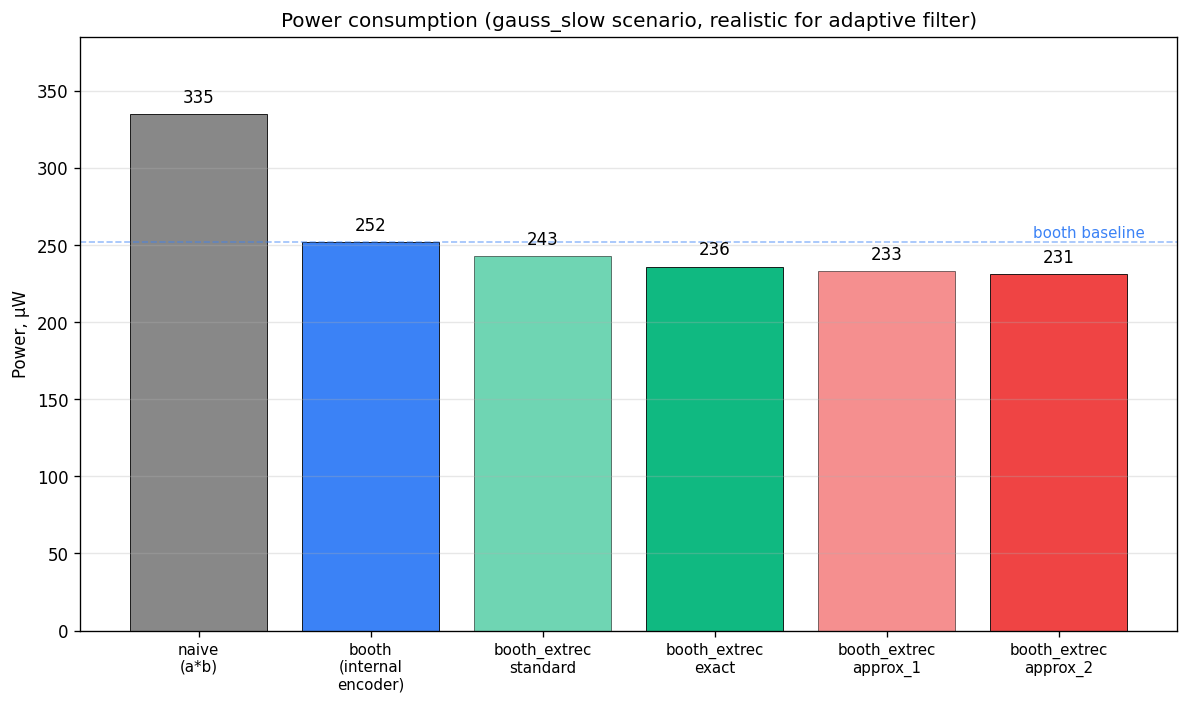
\includegraphics[width=0.6\textwidth]{power_dut_comparison_gauss_slow.png}
  \caption{Потребляемая мощность всех конфигураций в сценарии
           \texttt{gauss\_slow}; пунктиром отмечена линия базового
           умножителя Бута}
  \label{fig:power}
\end{figure}

Выделяется конфигурация \texttt{extrec\_standard}:
вынесенная архитектура с \textit{обычными} (не перекодированными)
коэффициентами потребляет \textit{больше} базового умножителя~---
из-за расширенного 24-битного регистра. Это измерение намеренно
включено в сравнение: оно разделяет два эффекта и подтверждает,
что экономию обеспечивают именно \textit{нулевые частичные
произведения}, а не сама архитектура выноса как таковая.

Результаты по всем четырём сценариям показаны на
рисунке~\ref{fig:power_scaling}. Видно, что сценарий \texttt{slow}
принципиально важен. Во-первых при более редком обновлении коэффициента 
модули ожидаемо потребляют 
меньше мощности относительно быстрого сценария, во-вторых видно, что в этом сценарии 
предлагаемый модуль проявляет себя лучше.
Это еще раз подтверждает факт, что уменьшение мощности вносит именно перекодировка. 


\begin{figure}[H]
  \centering
  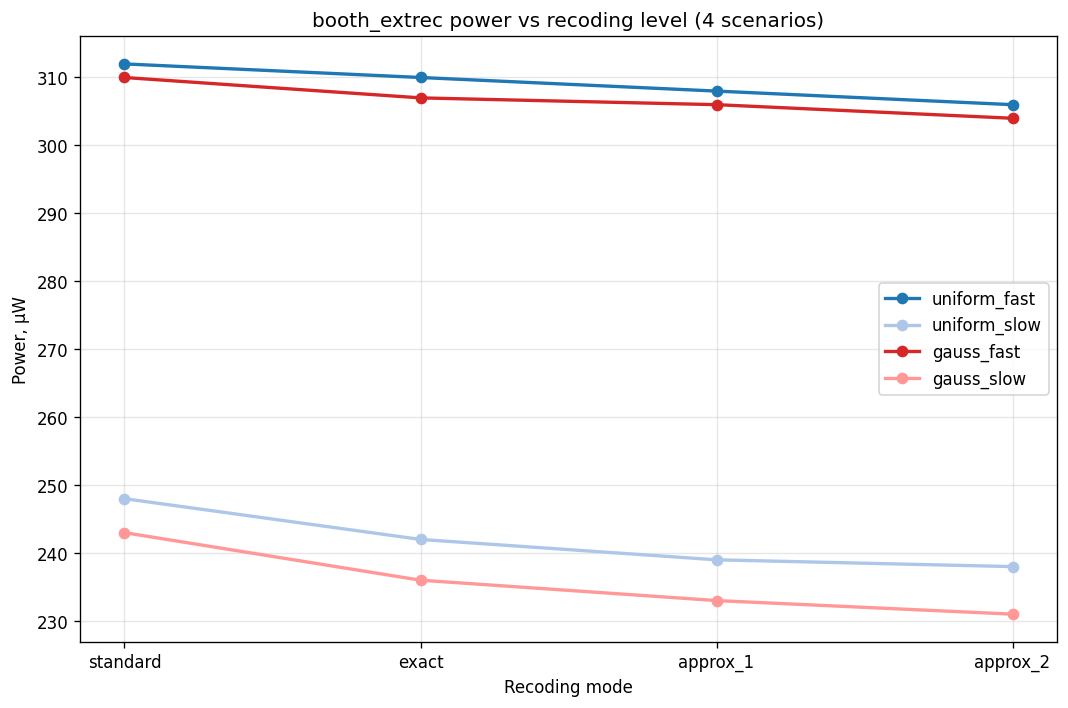
\includegraphics[width=0.88\textwidth]{power_extrec_vs_recoding_mode.png}
  \caption{Мощность предлагаемого умножителя по уровням перекодировки
           в 4~сценариях}
  \label{fig:power_scaling}
\end{figure}

\section{Точность}

Точность оценивалась на $10^6$~случайных парах операндов с гауссовым
и равномерным распределениями по трём метрикам:
\begin{itemize}
  \item \textbf{NMED}~--- нормированное среднее абсолютное отклонение
        результата~$\hat{p}$ от точного~$p$:
        $\mathrm{NMED} = \frac{1}{N} \sum |p - \hat{p}| / p_{\max}$.
  \item \textbf{MRED}~--- среднее относительное отклонение,
        нечувствительное к масштабу операндов:
        $\mathrm{MRED} = \frac{1}{N'} \sum |p - \hat{p}| / |p|$
        (по ненулевым~$p$).
  \item \textbf{SNR}~--- отношение мощности сигнала к мощности
        ошибки, дБ; наиболее естественная метрика для задач ЦОС.
\end{itemize}

Результаты представлены в таблице~\ref{tab:accuracy} и на
рисунке~\ref{fig:accuracy}.

\begin{table}[H]
  \caption{Метрики точности (гауссово распределение, $10^6$~пар)}
  \label{tab:accuracy}
  \centering
  \renewcommand{\arraystretch}{1.3}
  \begin{tabular}{lrrr}
    \toprule
    Режим & NMED & MRED & SNR, дБ \\
    \midrule
    \texttt{exact}     & $0$                   & $0$                   & $\infty$ \\
    \texttt{approx\_1} & $1{,}3 \cdot 10^{-6}$ & $3{,}8 \cdot 10^{-4}$ & 76{,}7   \\
    \texttt{approx\_2} & $2{,}2 \cdot 10^{-5}$ & $4{,}4 \cdot 10^{-3}$ & 52{,}3   \\
    \texttt{approx\_3} & $3{,}5 \cdot 10^{-4}$ & $3{,}8 \cdot 10^{-2}$ & 28{,}1   \\
    \texttt{approx\_4} & $1{,}5 \cdot 10^{-3}$ & $7{,}3 \cdot 10^{-2}$ & 15{,}6   \\
    \bottomrule
  \end{tabular}
\end{table}

\begin{figure}[H]
  \centering
  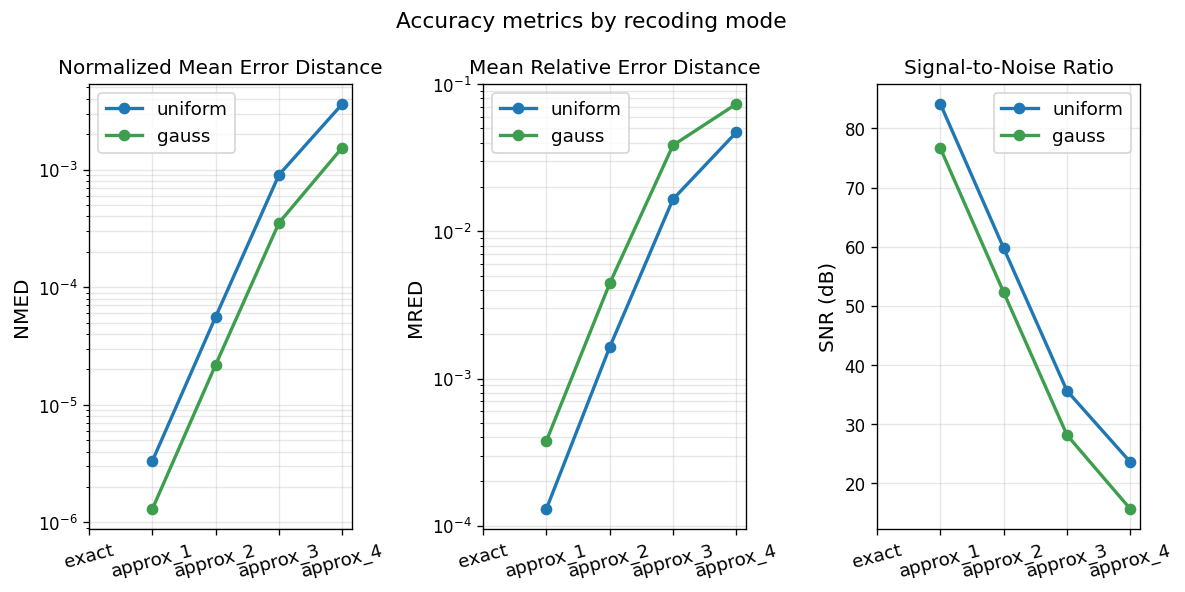
\includegraphics[height=0.3\textheight]{accuracy_nmed_mred_snr_main.png}
  \caption{Метрики точности по режимам перекодировки:
           NMED, MRED, SNR (кривые для равномерного
           и гауссового распределений)}
  \label{fig:accuracy}
\end{figure}

Режимы \texttt{approx\_3} и \texttt{approx\_4} демонстрируют
значительную погрешность (SNR менее 30~дБ) и не рекомендуются для
применения в большинстве задач ЦОС. Режимы \texttt{exact}~---
\texttt{approx\_2} обеспечивают NMED~$< 10^{-4}$~--- уровень,
считающийся хорошим в контексте приближённых вычислений~\cite{zhu2025}.

Систематическое смещение результата практически равно нулю во всех
режимах: ошибки $\mathrm{ED} = +1$ и $\mathrm{ED} = -1$ встречаются
с одинаковой частотой и компенсируют друг друга при усреднении. Это
исключает накопление систематической погрешности в адаптивном фильтре.

\section{Компромисс мощность/точность}

\begin{table}[H]
  \caption{Сводная таблица мощности и точности
           (сценарий \texttt{gauss\_slow})}
  \label{tab:tradeoff}
  \centering
  \renewcommand{\arraystretch}{1.3}
  \begin{tabular}{lrr}
    \toprule
    Режим & Изменение мощности & SNR, дБ \\
    \midrule
    \texttt{standard}  & $-1{,}6\%$ & $\infty$ \\
    \texttt{exact}     & $+0{,}4\%$ & $\infty$ \\
    \texttt{approx\_1} & $+1{,}6\%$ & 76{,}7   \\
    \texttt{approx\_2} & $+2{,}9\%$ & 52{,}3   \\
    \bottomrule
  \end{tabular}
\end{table}

Режим \texttt{approx\_2} является наиболее практически привлекательным:
экономия 2{,}9\% при SNR~$= 52{,}3$~дБ. Это значение превышает 
требования большинства аудио- и речевых приложений. Нулевое
систематическое смещение устраняет риск накопления погрешности.

Режим \texttt{exact} рекомендуется для задач, требующих
гарантированно точного результата при минимальном энергобонусе.

%% ============================================================
%%  ЗАКЛЮЧЕНИЕ
%% ============================================================
\chapter*{Заключение}
\addcontentsline{toc}{chapter}{Заключение}

В настоящей работе предложена, реализована и верифицирована архитектура
умножителя Бута radix-4 с вынесенным перекодировщиком для применения
в адаптивных FIR-фильтрах. Основные результаты:

\begin{enumerate}
  \item Выявлены два архитектурных препятствия прямого применения
        метода перекодирования из статьи~\cite{zhu2025} в параллельных умножителях
        FIR-фильтра: несовместимость переменной задержки последовательного
        умножителя с поточной обработкой и последовательная зависимость
        алгоритма перекодировки, исключающая его распараллеливание.

  \item Предложена архитектура с вынесенным перекодировщиком, в которой
        перекодировка коэффициента выполняется однократно при его
        обновлении; 24-битный результат хранится в регистре умножителя
        и без изменений используется на всех~$N$ тапах фильтра.

  \item Реализованы два RTL-модуля на Verilog: \texttt{mult\_booth}
        (исходный) и \texttt{mult\_booth\_extrec} (предлагаемый),
        поддерживающий пять режимов точности без каких-либо изменений
        аппаратной части.

  \item Построен воспроизводимый маршрут измерения площади и мощности
        целиком на открытых инструментах: Yosys, Icarus~Verilog,
        OpenSTA, библиотека NanGate45.

  \item Площадь предлагаемого умножителя не возрастает ($\Delta < 0{,}3\%$):
        уменьшение за счёт устранения логики кодирования компенсируется
        расширением регистра коэффициента.

  \item В наиболее реалистичном сценарии (\texttt{gauss\_slow})
        потребляемая мощность снижена на 2{,}9\% (режим \texttt{approx\_2})
        при SNR~$= 52$~дБ и нулевом систематическом смещении.
\end{enumerate}

\textbf{Перспективы дальнейших исследований:}
\begin{itemize}
  \item Оценка архитектуры на производственных библиотеках стандартных
        ячеек (TSMC 45~нм или аналог) для получения абсолютных значений
        мощности, применимых в промышленном контексте.
  \item Аппаратная RTL-реализация перекодировщика для сценариев с
        высокой частотой обновления коэффициентов.
  \item Интеграция предложенного умножителя в полную схему
        $N$-тапного адаптивного фильтра и оценка системного
        энергобюджета.
  \item Исследование масштабирования метода на умножители с большей
        разрядностью (24, 32~бита).
\end{itemize}

%% ============================================================
%%  СПИСОК ИСТОЧНИКОВ
%% ============================================================
\begin{thebibliography}{9}
\addcontentsline{toc}{chapter}{Список использованных источников}

\bibitem{booth1951}
  Booth~A.~D. A signed binary multiplication technique~//
  The Quarterly Journal of Mechanics and Applied Mathematics.~---
  1951.~--- Vol.~4, №~2.~--- P.~236--240.

\bibitem{zhu2025}
  Zhu~X., Li~H., Song~Y. Exact and approximate Radix-4 recoding
  multipliers for high-efficiency computation~//
  Microelectronics Journal.~--- 2025.~--- Vol.~157.~---
  DOI:~10.1016/j.mejo.2025.106579.

\bibitem{haykin2013}
  Haykin~S. Adaptive Filter Theory.~---
  5th ed.~--- Pearson, 2013.~--- 907~p.

\end{thebibliography}

\end{document}
